\documentclass{article}
\usepackage[margin=1in]{geometry} 
\usepackage{graphicx}
\usepackage{caption}
\usepackage{subcaption}
\usepackage{hyperref}
\usepackage{float}
\usepackage{epstopdf}
\usepackage{mathtools}
\usepackage{amsmath}
\usepackage{color}
\usepackage{array}

\setcounter{MaxMatrixCols}{20}

\providecommand{\e}[1]{\ensuremath{\times 10^{#1}}}


\title{\huge BME 4010 \\ Homework 2} 
\author{Samuel Tome}




\begin{document}
\maketitle
\captionsetup{width=1 \linewidth}


\begin{figure}[H]
\centering
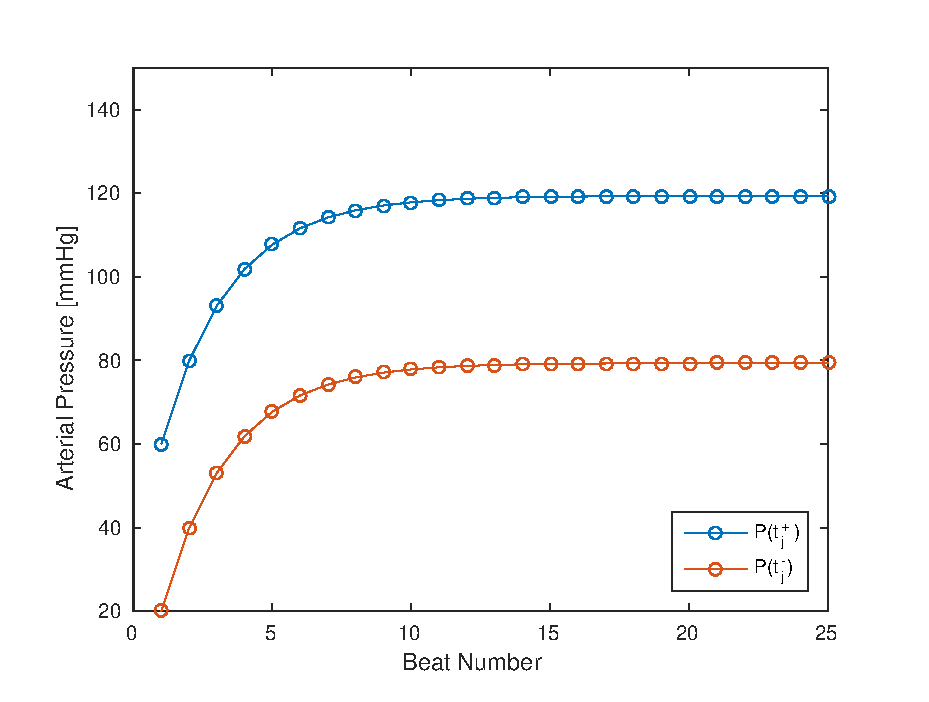
\includegraphics[width=4in]{figures/P_init20.eps}
\caption{Arterial pressure under normal conditions, with $P(t_1^-) = 20$ mmHg}
\end{figure}


\begin{figure}[H]
\centering
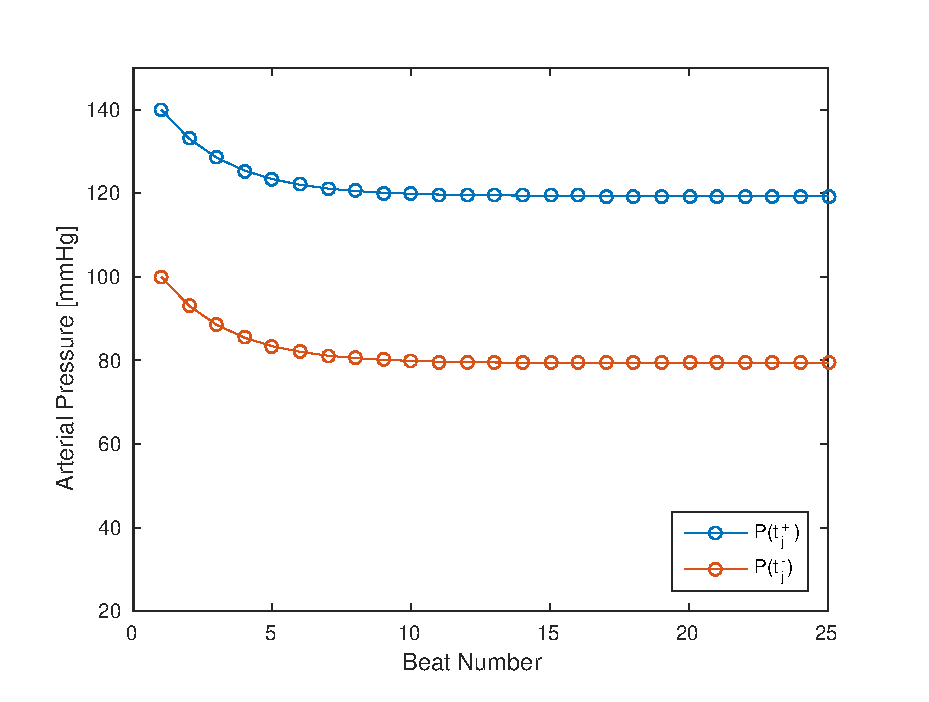
\includegraphics[width=4in]{figures/P_init100.eps}
\caption{Arterial pressure under normal conditions, with $P(t_1^-) = 100$ mmHg}
\end{figure}


\begin{figure}[H]
\centering
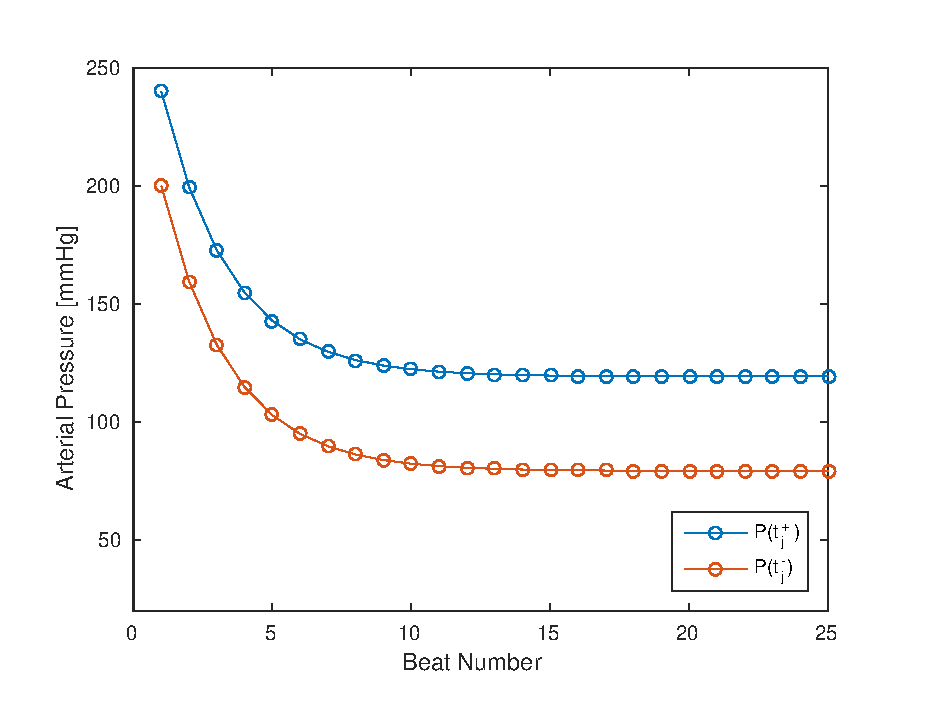
\includegraphics[width=4in]{figures/P_init200.eps}
\caption{Arterial pressure under normal conditions, with $P(t_1^-) = 200$ mmHg}
\end{figure}


\begin{figure}[H]
\centering
\begin{subfigure}{0.6\textwidth}
	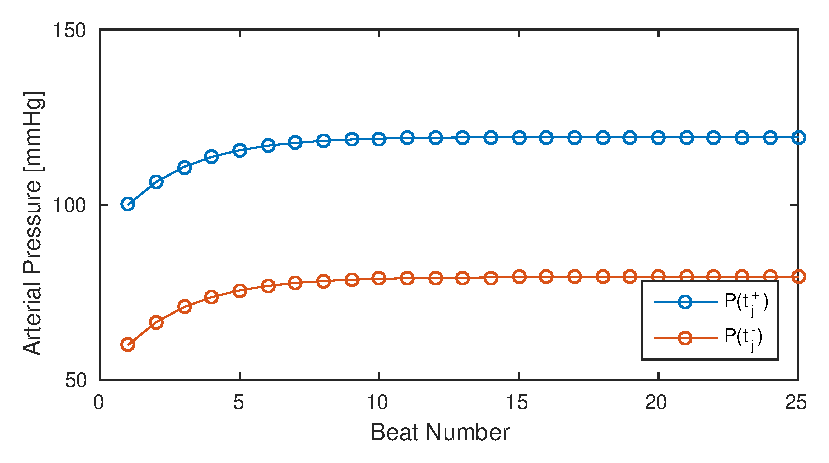
\includegraphics[width=\textwidth]{figures/P_A60.eps}
	\caption{$P(t_1^-) = 60$ mmHg}
\end{subfigure}

\vspace{20pt}
\begin{subfigure}{0.6\textwidth}
	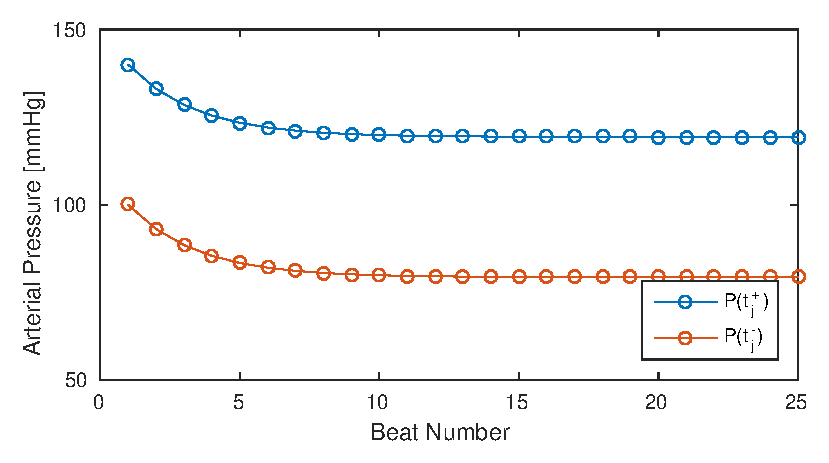
\includegraphics[width=\textwidth]{figures/P_A100.eps}
	\caption{$P(t_1^-) = 100$ mmHg}
\end{subfigure}
\caption{Arterial pressure with no mitral valve prolapse}
\end{figure}


\begin{figure}[H]
\centering
\begin{subfigure}{0.6\textwidth}
	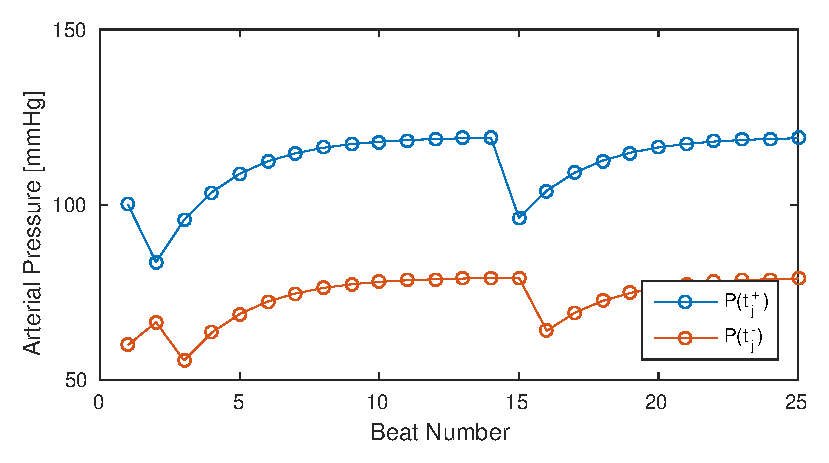
\includegraphics[width=\textwidth]{figures/P_B60.eps}
	\caption{$P(t_1^-) = 60$ mmHg}
\end{subfigure}

\vspace{20pt}
\begin{subfigure}{0.6\textwidth}
	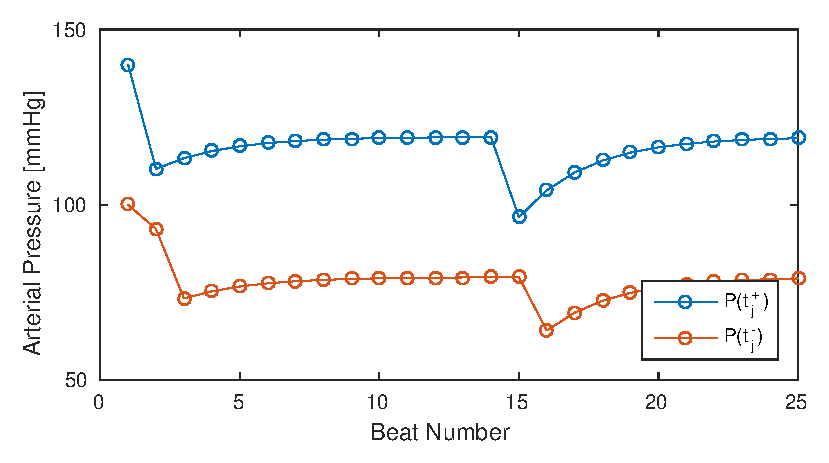
\includegraphics[width=\textwidth]{figures/P_B100.eps}
	\caption{$P(t_1^-) = 100$ mmHg}
\end{subfigure}
\caption{Arterial pressure with weak second and fifteenth beats}
\end{figure}



\begin{figure}[H]
\centering
\begin{subfigure}{0.6\textwidth}
	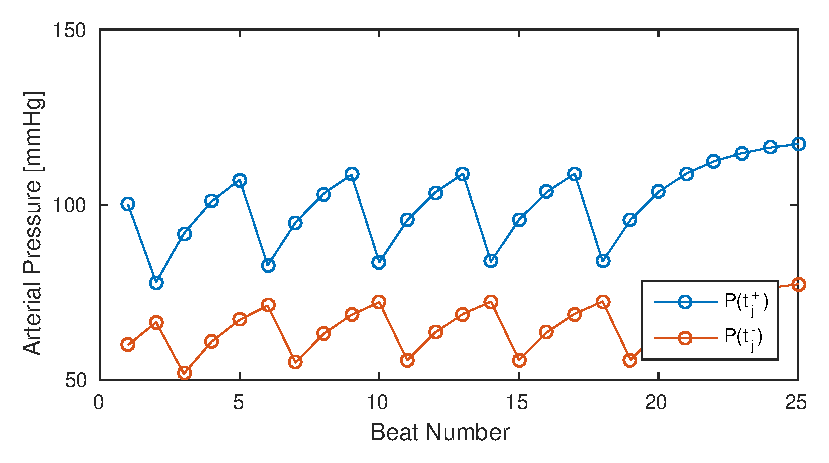
\includegraphics[width=\textwidth]{figures/P_C60.eps}
	\caption{$P(t_1^-) = 60$ mmHg}
\end{subfigure}

\vspace{20pt}
\begin{subfigure}{0.6\textwidth}
	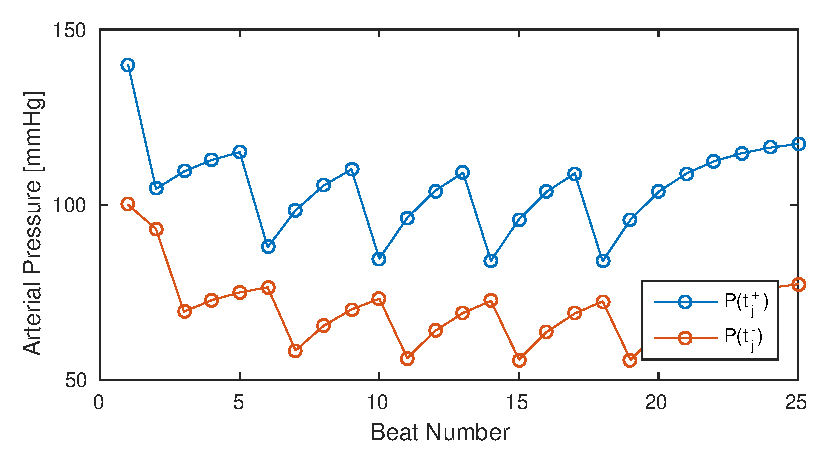
\includegraphics[width=\textwidth]{figures/P_C100.eps}
	\caption{$P(t_1^-) = 100$ mmHg}
\end{subfigure}
\caption{Arterial pressure with many weak beats}
\end{figure}




\end{document}